\documentclass{article}

\usepackage[utf8]{inputenc}
\usepackage{amsmath}
\usepackage{array}
\usepackage{listings}
\usepackage{xcolor}
\usepackage{graphicx}
\usepackage{tikz}
\usepackage{pgfplots}

\pgfplotsset{width=10cm,compat=1.9}

\lstset{
    language=Python,
    basicstyle=\ttfamily\small,
    keywordstyle=\color{blue},
    commentstyle=\color{gray},
    stringstyle=\color{purple},
    showstringspaces=false,
    breaklines=true,
    frame=single,
    numbers=left,
    numberstyle=\tiny\color{gray},
    captionpos=b
}

\title{Machine Learning - Week 1}
\author{ZVENC}
\date{December 2024}

\begin{document}

\maketitle

%\tableofcontents

\section{Introduction}
There are many problems that have been solved using rule-based algorithms, such as finding the shortest path between two points, sorting lists of items, etc. There are problems that cannot be solved this way because they are simply too complex; this is a problem area where machine learning excels. In simple terms, machine learning is a field concerned with teaching computers how to learn to do certain tasks. Machine learning is heavily relevant today, being used in various fields such as healthcare, scientific research, social media, manufacturing, etc.

\subsection{Types of Machine Learning Approaches}
Machine Learning algorithms can be categorized into two main types:

\begin{enumerate}

\item Supervised Learning
\item Unsupervised Learning

\end{enumerate}

\noindent While there are other types of machine learning, these two are the most relevant at this stage.

\subsubsection{Supervised Learning ($x \rightarrow y$)}
This approach to machine learning involves giving the computer a number of examples to learn from in the form of input-output pairs. The output represents what is expected given a particular input. The computer then learns from these input-output pairs and tries to guess the correct output for an input that it has never seen before.

For example let's say you had a plot of house prices against size for about 15 houses. The goal would be to get the computer to estimate the price of a house based on its size, even for houses not explicity represented in the dataset. This is called a \textit{'regression problem'}, and the relationships could either be linear, polynomial, etc.

Another example is breast cancer detection. A model can learn to predict whether a tumor is cancerous based on its size. It can be provided with a plot of patient age against tumor size with the malignant and benign tumors marked on the plot. The model might the attempt to create a boundary to identify malignant tumors. In this example, the model only has to guess between two possible output classes, 'benign' or 'malignant'. This is what's known as a \textit{'classification problem'}. Unlike regression, classification requires the model to predict the correct value from a finite set of classes, not necessarily just two, like in the example. A model could also be designed to detect different classes of malignant tumors, in which case the classes could be 'benign', 'malignant-type-1', and 'malignant-type-2'.

\subsubsection{Unsupervised Learning ($x$)}
With supervised learning, a model learns from data labeled with 'correct answers'. In contrast, unsupervised learning involves providing the model with unlabeled data and tasking it with finding any patterns or structures hidden within the data. Let's say we have another patient age vs tumor size plot except the points aren't labeled. A model might try to group the points into categories or \textit{'clusters'}. This is type of supervised learning algorithm called a \textit{'clustering algorithm'}. Google News employs this algorithm to group related news articles. Achieving this with supervised learning is unfeasible for obvious reasons. Other unsupervised learning algorithms include \textit{'anomaly detection'} and \textit{'dimensionality reduction'}.

\subsection{Terminology}

\begin{enumerate}

\item Training Set: Data used to train the model
\item Input Variable ($x$): The input provided to the model in the training set. Also called \textit{'feature'} or \textit{'input feature'}.
\item Output Variable ($y$):  The output correct output provided to the model in the training set. Also called the \textit{'target'} variable.
\item Training Example ($x^{(i)}, y^{(i)}$): This is an input output pair from the training set. The superscript '$i$' represents the position of the training example in the training set, for instance, in a table.
\item Total Number of Training Examples ($m$): I believe this is self-explanatory.

\end{enumerate}

\subsection{Linear Regression Model}
The training set, which contains the input features and output targets, is fed into the supervised learning algorithm. The algorithm then produces a function (historically called a hypothesis) that it then uses to estimate an output for any given input. That function, also called a model, takes  in a feature, $x$, and then produces and estimate, $\hat{y}$. Note the difference between $y$ and $\hat{y}$; $y$ is the target/true value in the training set, while $\hat{y}$ is an estimate of $y$. A linear regression model takes on the form:

\[ f_{w,b}(x) = wx + b\]

% w and b will be defined later
\noindent For the sake of convenience, $f_{w,b}(x)$ will be written as $f(x)$. If the features and targets were plot on a graph, the algorithm would generate a best-fit line for the plot which would be represented by that equation.
\vspace{5mm}

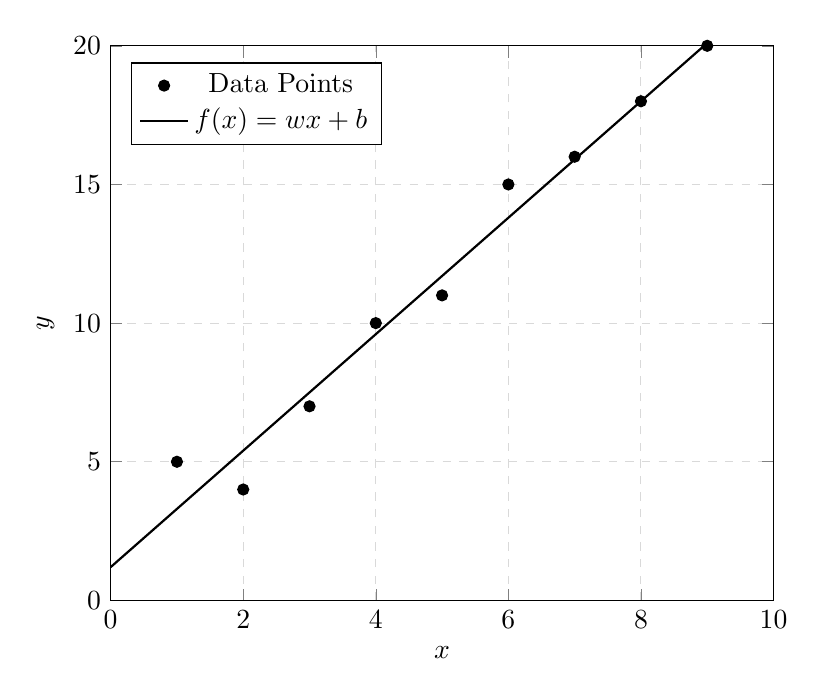
\begin{tikzpicture}
    \begin{axis}[
        xlabel={\( x \)},
        ylabel={\( y \)},
        xmin=0, xmax=10,
        ymin=0, ymax=20,
        xtick={0,2,4,6,8,10},
        ytick={0,5,10,15,20},
        legend pos=north west,
        grid=major,
        grid style={dashed, gray!30},
    ]
    
    \addplot[
        only marks,
        mark=*,
        mark size=2pt,
    ] coordinates {
        (1, 5)
        (2, 4)
        (3, 7)
        (4, 10)
        (5, 11)
        (6, 15)
        (7, 16)
        (8, 18)
        (9, 20)
    };
    \addlegendentry{Data Points}
    
    \addplot[
        domain=0:10,
        samples=2,
        thick
    ] {2.1*x + 1.2};
    \addlegendentry{$f(x) = wx + b$}
    
    \end{axis}
\end{tikzpicture}

\noindent This is one-variable or \textit{univariate} linear regression, which means there's a single feature for each data point. Using the house price example, it is possible to take other factors into consideration rather than just the size of the house such as number of bedrooms, location, etc.

\subsubsection{Linear Regression Implementation in Python}
A linear regression model can be implemented in python using \texttt{numpy} and \texttt{matplotlib}. Here is a linear regression model for predicting house prices based on size using this training set:

\begin{center}
\centering
\begin{tabular}{|c|c|} 
\hline
\textbf{$x$} & \textbf{$y$} \\ 
\hline
1.0 & 300.0 \\ 
\hline
2.0 & 500.0 \\ 
\hline
3.0 & 580.0 \\ 
\hline
4.0 & 830.0 \\ 
\hline
5.0 & 900.0 \\ 
\hline
6.0 & 1100.0 \\ 
\hline
\end{tabular}
\center {House size in 1000$ft^2$($x$) and house price in \$1000($y$)}
\end{center}

\begin{lstlisting}[caption={Python Code for Linear Regression}]
import numpy as np
import matplotlib.pyplot as plt

# feature array
x_train = np.array([1.0, 2.0, 3.0, 4.0, 5.0, 6.0])

# target array
y_train = np.array([300.0, 500.0, 580.0, 830.0, 900.0, 1100.0 ])

m = x_train.shape # number of training examples
w = 170 # weight
b = 100 # bias

def compute_model_output(x, w, b):
    """
    Computes the prediction of a linear model
    args:
        x (ndarray (m,))    : data, size m
        w, b (scalar)       : model parameters
    returns:
        f_wb (ndarray (m,)) : model prediction
    """
    m = x.shape[0]
    f_wb = np.zeros(m)
    for i in range(m):
        f_wb[i] = w * x[i] + b
    return f_wb

x_i = 1.2
cost_1200sqft = w * x_i + b
print(f"cost of a 1200 sq. ft. house is predicted to be ${cost_1200sqft:.0f}K")

f_wb = compute_model_output(x_train, w, b)
plt.scatter(x_train, y_train, marker='.', c='black')
plt.plot(x_train, f_wb, c='black', label='model prediction')
plt.xlabel("size of house in 1000s sq. ft.")
plt.ylabel("price of house in $1000s")
plt.show()
\end{lstlisting}
\vfill

\begin{figure}
\centering
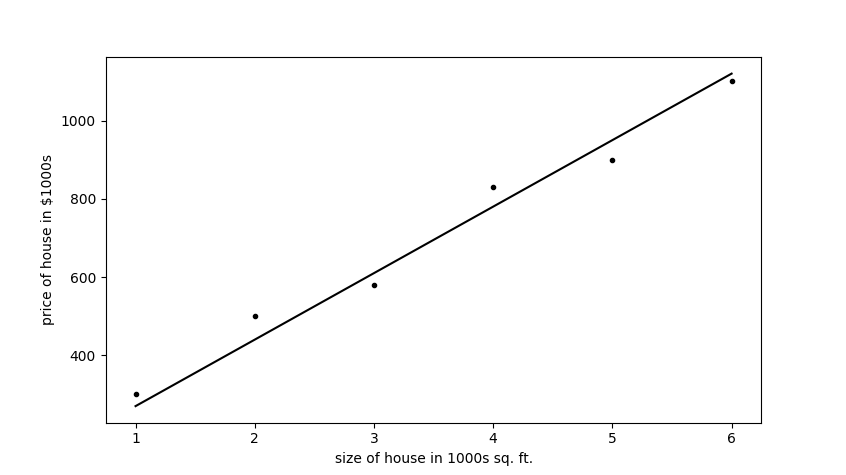
\includegraphics[width=1\textwidth]{linear_regression.png}
\end{figure}

\begin{lstlisting}[caption={Code Output}]
# cost of a 1200 sq. ft. house is predicted to be $304K
\end{lstlisting}

\noindent In the implementation, the features (\texttt{x\_train}) and targets (\texttt{y\_train}) are stored in respective \texttt{numpy} arrays. The number of training examples is obtained by finding the number of items in the features array, using the array's \texttt{.shape} method (it returns a tuple containing the size of the array along each dimension). The \texttt{compute\_model\_output} function creates an array containing the model's estimations of training set's targets, which is used to generate the graph. The weight and bias were initially arbitrarily set but later adjusted to fit the plots on the generated graph. With the accepted weight and bias, the model is used to provide an estimate of the price of a house that is 1200$ft^2$, which is \$304,000.

\subsubsection{Cost Function}
In order to adjust the parameters of a linear regression model appropriately, it is necessary to have a reliable way to deduce how well the model is performing on the training data. This is acheived through the \textit{cost function}. This function compares the predictions of the model to the targets and outputs a number that is used to quantify the model's performance. The most commonly used linear regression cost function is called the \textit{Squared Error Cost Function}. Recall that

\[
\hat{y} =  f_{w, b}(x) \quad \textrm{and} \quad f_{w, b}(x) = wx + b
\]

\noindent where $\hat{y}$ is the model's prediction for a given feature. The squared cost function can then be expressed as

\[ J(w, b) = \frac{1}{2m}\sum^{m}_{i = 1}{ ({ \hat{y}^{(i)} - y^{(i)} })^2 }\]

\noindent where $J(w, b)$ is the cost function, $m$ is the number of training examples, $y^{(i)}$ is a feature, and $\hat{y}^{(i)}$ is a prediction.

\noindent The goal is to make the output of the cost function as small as possible

\[\min_{w, b}J(w, b)\]

\noindent as the size of the output directly reflects the variance between the model's predictions and the target values. Thus, it should be kept to a minimum. 

Given $y = x$, if $b$ is set to 0 and $J$ is plot against $w$ for different values of $w$, observing the resulting parabola might help build some intuition about the behavior of the cost function.

\noindent For example, if $w = 1$, $f_{w}(x) = x$ therefore, $y = f_{w}(x)$. This implies,
\begin{align*}
&J(1) \quad=\quad \frac{1}{2m}\sum^m_{i=1}{ (wx^{(i)} - y^{(i)})^2 } \\
&J(1) \quad=\quad \frac{1}{2\times3}[(1-1) + (2-2) + (3-3)] \quad=\quad 0 \\
\end{align*}

\noindent Repeating this process for more values of $w$ we get:

\begin{center}
\centering
\begin{tabular}{|c|c|}
\hline
\textbf{$w$} & \textbf{$J(w)$} \\
\hline
0 & $\approx 2.3$ \\
\hline
0.5 & $\approx 0.58$ \\
\hline
1.5 & $\approx 0.58$ \\
\hline
2 & $\approx 2.3$ \\
\hline
\end{tabular}
\end{center}

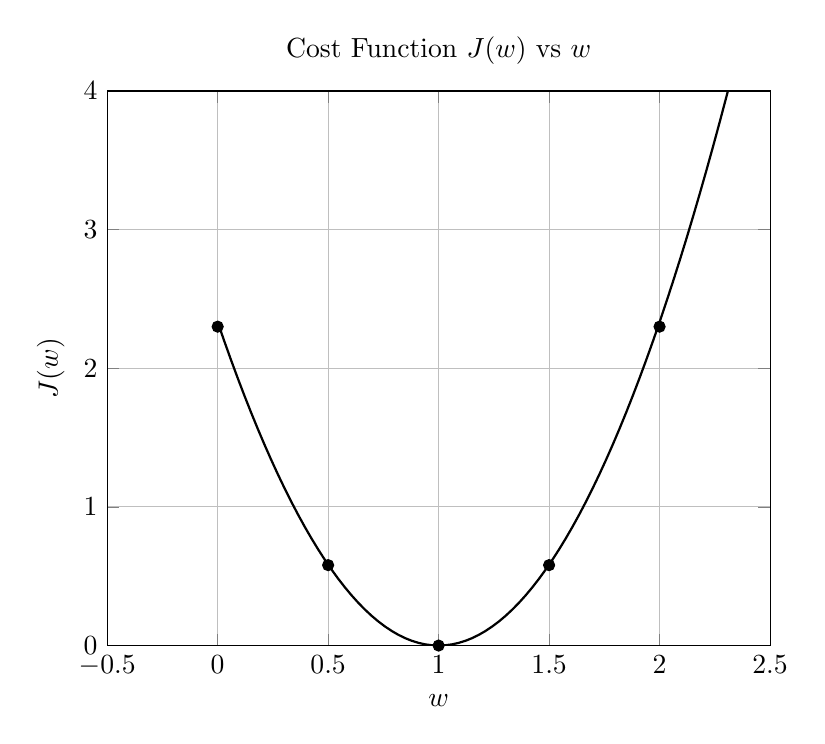
\begin{tikzpicture}
\begin{axis}[
	title={Cost Function $J(w)$ vs $w$},
	xlabel={$w$},	
	ylabel={$J(w)$},
	grid=major,
	xmin=-0.5, xmax=2.5,
	ymin=0, ymax=4,
	xtick={-0.5,0,0.5,1,1.5,2,2.5},
	ytick={0,1,2,3,4}
]

\addplot[
	only marks,
	mark=*,
	mark size=2pt,
] coordinates {
	(0, 2.3)
	(0.5, 0.58)
	(1, 0)
	(1.5, 0.58)
	(2, 2.3)
};

\addplot[
	domain=0:3,
	samples=100,
	thick
] {((x - 1)^2 + (2*x - 2)^2 + (3*x - 3)^2) / 6};
\end{axis}	
\end{tikzpicture}

\end{document}
